\documentclass{article}

\usepackage[margin=1in]{geometry}
\usepackage{graphicx}
\graphicspath{ {images/} }

\begin{document}

\begin{flushright}
Kyle Pierson, Johnny Le, and Pierce Darragh\\
CS 6150\\
Final Report\\
December 16, 2017
\end{flushright}

\section{Introduction}
  For our project, we analyzed and improved upon the work done in the 2003 paper ``Maximizing the Spread of Influence through a Social Network'' by Kempe, Kleinberg, and Tardos \cite{kempe}. The paper discusses methods for selecting a group of nodes within a social network with the goal of maximizing the ``influence'' that can be spread through the network. The authors detail two models for simulating diffusion of influence within the network --- a \emph{linear threshold model} and an \emph{independent cascade model} --- and introduce a greedy algorithm for selecting the set of nodes which will maximize the spread of influence through the network. However, the greedy algorithm is very slow; on a graph with only around 7,000 nodes, it took about four minutes per iteration.

  In this report, we propose a new heuristic for selecting a set of influential nodes with the caveat that they are not guaranteed to be the most influential. Rather, we make some concessions to increase performance while attempting to minimize the loss in accuracy incurred by our approximation. We show that our approximation performs reasonably well, leading to only a marginal drop in accuracy with a significant improvement in time.

\section{Implementation}

  \subsection{Graph Representation}
    We used the SNAP format \cite{snap} for representing our graph.  SNAP is a fast and scalable graph-manipulation library written in C++ by Prof. Jure Leskovec from Stanford University.  In order to leverage the flexibility of Python, we used the Snap.py interface, which provides nearly all of the functionality of the base SNAP.  Stanford also provides a collection of large network datasets, from which we chose a network of reasonable size on which to run our experiments.  The network we chose contained 7,115 nodes and 103,698 directed edges.  We chose to use directed graphs because we felt they most accurately modelled the structure of many social networks.  The direction of the edges captures the notion of one user ``following'' another, e.g. if Alice follows Bob, then Bob influences Alice, but Alice does not necessarily influence Bob.

    On loading the network, each node was assigned an ``active'' attribute, which was initialized to 0.  It was also assigned a ``threshold'' attribute (applicable only to the linear threshold diffusion model), which was drawn randomly from a uniform distribution.  Each edge was assigned a ``weight'' attribute, which would eventually represent either a weight or a probability for the linear threshold or independent cascade model, respectively.

  \subsection{Linear Threshold Model}
    The first diffusion model that can be used for measuring influence is the linear threshold model.  In this model, a node $v$ will become active if a weighted combination of its influencing neighbors surpasses the activation threshold of $v$.  The threshold of $v$ is chosen uniformly at random on the interval $[0, 1]$.  The weighted combination is given by $\sum_{w \in \Lambda(v)} a_w b_{v,w}$, where $\Lambda(v)$ represents the neighbors of $v$ with directed edges into $v$.  The edge weights $b_{v,w}$ must also adhere to the property that $\sum_{w \in \Lambda(v)} b_{v,w} \leq 1$.

    For each node $v$ in the graph, edges directed toward $v$ were assigned a weight corresponding to $\frac{1}{D(v)}$ where $D(v)$ represents the total number of edges which were directed towards $v$. For each node $u$ which was activated, each neighbor $v \in \Gamma(u)$ had its activation determined by the equation $t = \frac{|\{a \in \Gamma(v), a \textrm{ is active}\}|}{|\Gamma(v)|}$. If $t > \theta_v$, then $v$ will become activated and added to a stack to be iterated over in the future.

  \subsection{Independent Cascade Model}
    The second diffusion model talked about in the paper is the independent cascade model. In this model, when a node $v$ first becomes active, it attempts to activate its neighbors $w \in \Gamma(v)$ with probability $p_{v, w}$. Each node is given only one chance to influence each of its neighbors, and the process repeats until there are no more activations possible.

    The paper is not clear in defining the probability parameter $p_{v, w}$. We experimented with both a fixed probability to be used for all edges in the graph as well as a uniform random distribution over a specified range. We document the outcomes of these experiments in the results section.

  \subsection{Greedy Algorithm}
    The paper utilized an inefficient algorithm that involved iterating through the entire graph and calculating a perceived influence starting from each node. Once completed, the node with the greatest perceived influence from the simulation would be marked as activated and added to the set, and all of the nodes which were activated during the simulation would remain active. For each subsequent iteration of the algorithm, only the subgraph of un-activated nodes were considered. The perceived influences of these nodes were calculated, and again the node with the greatest influence would be activated and added to the set. The process iterated $k$ times.

  \subsection{Graph Partitioning Heuristic}
    We developed a new heuristic designed to deliver approximately equivalent results to the greedy algorithm, but in significantly less time. For each iteration of this heuristic, the graph was divided into $k$ subgraphs by means of the METIS library?s partitioning function \cite{metis}. Each subgraph was searched for the node $v$ with the highest influence, and we computed the total influence for the graph as the sum of these influences. We chose this method because we wanted to increase the efficiency of the algorithm in two ways: first, we wanted to not use a greedy approach, since we figured that was a performance bottleneck; and second, we wanted to divide the network into subgraphs by cutting between less-connected nodes to promote searching over denser sub-networks. We repeated this process ten times, and the mean influence over each of the $k$ cycles was recorded.

\pagebreak
\section{Results}
  For the greedy algorithms below, $k$ represents the number of nodes with the best perceived influence. Each iteration recorded the influence of one additional node, and successive trials built on the work of their predecessors.
  
  For the partitioning heuristic, $k$ represents the number of subgraphs created. Each run recorded the average influence generated across ten independent trials with a given $k$ value.
  
  Each iteration for all data is accompanied by a list of which nodes were selected to maximize the spread of influence with the given parameters.

  \subsection{Linear Threshold Model}
  
    \begin{figure}[h]
      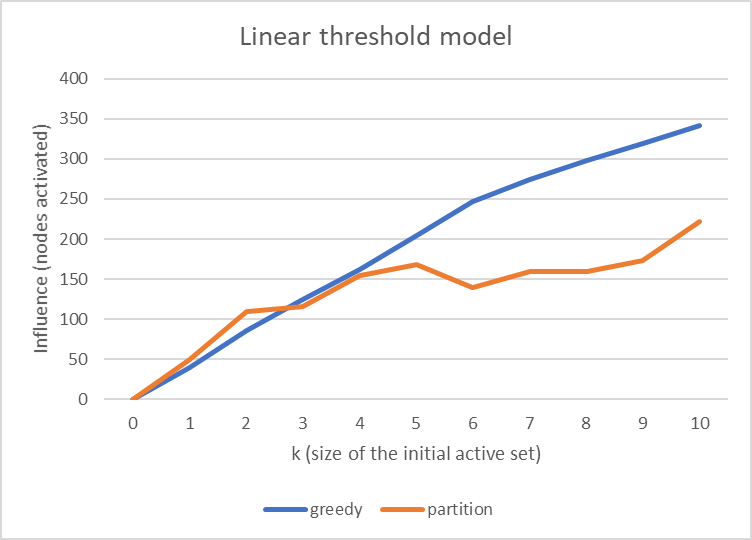
\includegraphics{linear}
      \centering
    \end{figure}
    
    \subsubsection{Greedy}
      
      \textbf{Runtime:} $2852$ seconds ($\approx 47.5$ minutes)

      \begin{center}
        \begin{tabular}{|lll|}
          \hline
          $k$ & influence & max set (nodes selected for spreading influence) \\
          \hline
          1  & 40  & [2565] \\
          2  & 86  & [2565, 11] \\
          3  & 125 & [2565, 11, 457] \\
          4  & 162 & [2565, 11, 457, 766] \\
          5  & 204 & [2565, 11, 457, 766, 1166] \\
          6  & 247 & [2565, 11, 457, 766, 1166, 5802] \\
          7  & 274 & [2565, 11, 457, 766, 1166, 5802, 5800] \\
          8  & 298 & [2565, 11, 457, 766, 1166, 5802, 5800, 2688] \\
          9  & 319 & [2565, 11, 457, 766, 1166, 5802, 5800, 2688, 1151] \\
          10 & 341 & [2565, 11, 457, 766, 1166, 5802, 5800, 2688, 1151, 6] \\
          \hline
        \end{tabular}
      \end{center}
    
    \pagebreak
    \subsubsection{Averaged Partitioning}
      
      \textbf{Runtime:} $234$ seconds ($\approx 4$ minutes)

      \begin{center}
        \begin{tabular}{|lll|}
          \hline
          $k$ & avg. inf. & max set (nodes selected for spreading influence) \\
          \hline
          1  & 50.0  & [3453] \\
          2  & 110.0 & [3453, 5189] \\
          3  & 116.0 & [3453, 5189, 7047] \\
          4  & 155.0 & [3453, 5189, 7047, 4037] \\
          5  & 168.0 & [3453, 5189, 7047, 4037, 3642] \\
          6  & 140.0 & [3453, 5189, 7047, 4037, 3642, 2565] \\
          7  & 160.0 & [3453, 5189, 7047, 4037, 3642, 2565, 2256] \\
          8  & 159.0 & [3453, 5189, 7047, 4037, 3642, 2565, 2256, 8] \\
          9  & 173.0 & [3453, 5189, 7047, 4037, 3642, 2565, 2256, 8, 1549] \\
          10 & 222.0 & [3453, 5189, 7047, 4037, 3642, 2565, 2256, 8, 1549, 11] \\
          \hline
        \end{tabular}
      \end{center}
    
  \subsection{Independent Cascade Model}
  
    \begin{figure}[h]
      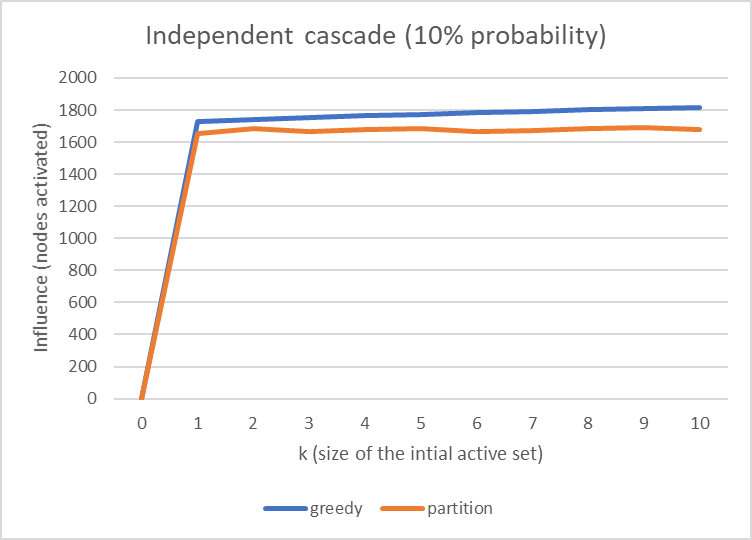
\includegraphics{cascade}
      \centering
    \end{figure}
    
    \pagebreak
    \subsubsection{Greedy}
      
      \textbf{Runtime:} $8052$ seconds ($\approx 2.25$ hours)

      \begin{center}
        \begin{tabular}{|lll|}
          \hline
          $k$ & influence & max set (nodes selected for spreading influence) \\
          \hline
          1  & 1728 & [1234] \\
          2  & 1741 & [1234, 11] \\
          3  & 1751 & [1234, 11, 59] \\
          4  & 1763 & [1234, 11, 59, 457] \\
          5  & 1774 & [1234, 11, 59, 457, 128] \\
          6  & 1783 & [1234, 11, 59, 457, 128, 766] \\
          7  & 1793 & [1234, 11, 59, 457, 128, 766, 7086] \\
          8  & 1802 & [1234, 11, 59, 457, 128, 766, 7086, 10] \\
          9  & 1810 & [1234, 11, 59, 457, 128, 766, 7086, 10, 312] \\
          10 & 1818 & [1234, 11, 59, 457, 128, 766, 7086, 10, 312, 2688] \\
          \hline
        \end{tabular}
      \end{center}
    
    \subsubsection{Averaged Partitioning}
      
      \textbf{Runtime:} $72$ seconds ($\approx 1$ minute)

      \begin{center}
        \begin{tabular}{|lll|}
          \hline
          $k$ & avg. inf. & max set (nodes selected for spreading influence) \\
          \hline
          1  & 1651.7 & [3453] \\
          2  & 1683.4 & [3453, 5189] \\
          3  & 1668.0 & [3453, 5189, 7047] \\
          4  & 1677.9 & [3453, 5189, 7047, 4037] \\
          5  & 1685.9 & [3453, 5189, 7047, 4037, 3642] \\
          6  & 1668.4 & [3453, 5189, 7047, 4037, 3642, 2565] \\
          7  & 1674.6 & [3453, 5189, 7047, 4037, 3642, 2565, 2256] \\
          8  & 1685.3 & [3453, 5189, 7047, 4037, 3642, 2565, 2256, 8] \\
          9  & 1690.1 & [3453, 5189, 7047, 4037, 3642, 2565, 2256, 8, 1549] \\
          10 & 1676.9 & [3453, 5189, 7047, 4037, 3642, 2565, 2256, 8, 1549, 11] \\
          \hline
        \end{tabular}
      \end{center}
  
  \section{References}
    \begin{thebibliography}{3}
      \bibitem{kempe}
        D. Kempe, J. Kleinberg, and \'E. Tardos, ``Maximizing the spread of influence through a social network,'' \textit{Proceedings of the Ninth ACM SIGKDD International Conference on Knowledge Discovery and Data Mining - KDD 03}, 2003.

      \bibitem{snap}
        J. Leskovec and R. Sosic. \textit{Snap.py: SNAP for Python}. \\\texttt{http://snap.stanford.edu}, 2014.

      \bibitem{metis}
      G. Karypis. \textit{METIS - Serial Graph Partitioning and Fill-reducing Matrix Ordering}. \\\texttt{http://glaros.dtc.umn.edu/gkhome/views/metis}. 2013.

    \end{thebibliography}


\end{document}
